% Complete Section 2.3, PDF 22-25 / printed 12-15, ending before Section 2.4.
% Original Fraktur Z/B are represented by user-approved mathcal Z/B.
% block: simplicial-chain-heading page:22 type:section
\subsection{\BT{Example: The simplicial chain complex}{Example: 单纯链复形}}\label{sec:simplicial-chain-complex}

% block: simplicial-complex-definition page:22 type:ordinary-paragraph
\BT{A classical example of a chain complex, the one which accounts for much of the terminology, is the \emph{simplicial chain complex} associated to a simplicial complex. By a $k$-dimensional simplex in some Euclidean space $\mathbb R^n$ we mean the convex hull $f$ of $k+1$ points $x_0,\ldots,x_k$, called the vertices of $f$, which we assume to be in general position in $\mathbb R^n$. Each nonempty subset of the vertex set of $f$ determines a simplex of some dimension $\leq k$, which is called a face of $f$. A simplicial complex is a finite set $\mathcal S$ of simplices in $\mathbb R^n$ such that (1) whenever a simplex belongs to $\mathcal S$, each of its faces also belongs to $\mathcal S$, and (2) if $f$ and $g$ are two simplices in $\mathcal S$, then their intersection $f\cap g$ is either empty or a face of $f$ and of $g$. The underlying space of the simplicial complex, that is, the subset of $\mathbb R^n$ obtained as the union of the simplices, may be a polyhedral domain, a piecewise flat manifold, or a more complicated set. The dimension of the simplicial complex is the highest dimension of any of its simplices, and a simplicial complex of dimension $k$ is said to be \emph{pure} if every simplex belonging to it is contained in a simplex of dimension $k$.}{链复形的一个经典例子, 也是许多术语的来源, 是与单纯复形相伴的\emph{单纯链复形}. 所谓某个 Euclidean 空间 $\mathbb R^n$ 中的 $k$ 维单纯形, 是指 $k+1$ 个点 $x_0,\ldots,x_k$ 的凸包 $f$; 这些点称为 $f$ 的顶点, 并假定它们在 $\mathbb R^n$ 中处于一般位置. $f$ 的顶点集的每个非空子集都确定一个维数 $\leq k$ 的单纯形, 称为 $f$ 的一个面. 单纯复形是 $\mathbb R^n$ 中单纯形的有限集合 $\mathcal S$, 满足 (1) 只要一个单纯形属于 $\mathcal S$, 它的每个面也都属于 $\mathcal S$; (2) 若 $f$ 和 $g$ 是 $\mathcal S$ 中的两个单纯形, 则它们的交 $f\cap g$ 或者为空, 或者同时是 $f$ 和 $g$ 的一个面. 单纯复形的底空间, 即这些单纯形的并所形成的 $\mathbb R^n$ 的子集, 可以是多面体区域, 分片平坦流形, 或更复杂的集合. 单纯复形的维数是其中所有单纯形维数的最大值; 若一个 $k$ 维单纯复形中的每个单纯形都包含在某个 $k$ 维单纯形中, 则称该单纯复形是\emph{纯的}.}

% block: oriented-simplices-figure page:23 type:figure
\begin{figure}[htbp]\centering
\includegraphics[page=23,trim=105bp 566bp 56bp 62bp,clip,width=.72\linewidth]{../input/source/Finite Element Exterior Calculus.pdf}
\caption{\BT{Oriented simplices of dimensions 1, 2, and 3.}{维数为 1, 2 和 3 的定向单纯形.}}\label{fig:oriented-simplices}
\end{figure}

% block: pure-complex-triangulation page:23 type:ordinary-paragraph
\BT{The notion of a pure simplicial complex is essentially the same as that of a triangulation of the underlying space. More precisely, a finite set of $n$-dimensional simplices constitute a triangulation of their union if and only if they, together with all their faces of all dimensions, form a pure $n$-dimensional simplicial complex.}{纯单纯复形的概念, 实质上与其底空间的剖分这一概念相同. 更准确地说, 一个由 $n$ 维单纯形组成的有限集合构成其并的一个剖分, 当且仅当这些单纯形连同它们所有维数的全部面, 构成一个纯 $n$ 维单纯复形.}

% block: simplex-orientation page:23 type:ordinary-paragraph
\BT{A simplex may be \emph{oriented} by selecting an ordering of its vertices, with the understanding that two orderings are equivalent if they differ by an even permutation. Thus every simplex of dimension $k>0$ has two possible orientations. See Figure~\ref{fig:oriented-simplices}. We shall write $[x_0,\ldots,x_k]$ for the simplex with vertices $x_0,\ldots,x_k$ endowed with the orientation determined by the given ordering of the vertices. We may (and shall) designate a preferred orientation for all the simplices in the simplicial complex $\mathcal S$ by fixing an ordering of the set of all the vertices of the simplicial complex, e.g., lexicographic ordering. The oriented simplex $[x_0,\ldots,x_k]$ is then said to be of \emph{positive orientation} if the vertex sequence $x_0,\ldots,x_k$, or some even permutation of it, is in increasing order.}{可以通过选定顶点的一个次序为单纯形\emph{定向}, 其中约定: 若两个次序相差一个偶置换, 则认为它们等价. 因此, 每个维数 $k>0$ 的单纯形都有两种可能的定向. 见 Figure~\ref{fig:oriented-simplices}. 我们用 $[x_0,\ldots,x_k]$ 表示以 $x_0,\ldots,x_k$ 为顶点, 并配备由给定顶点次序确定的定向的单纯形. 固定单纯复形全部顶点集合的一个次序, 例如字典序, 就可以 (而且我们也将这样做) 为单纯复形 $\mathcal S$ 中的所有单纯形指定一个优先选用的定向. 此时, 若顶点序列 $x_0,\ldots,x_k$ 或它的某个偶置换按递增次序排列, 则称定向单纯形 $[x_0,\ldots,x_k]$ 为\emph{正定向的}.}

% block: simplicial-chain-definition page:23 type:ordinary-paragraph
\BT{Let $\mathcal S$ be a simplicial complex in $\mathbb R^n$ and denote by $\Delta_k(\mathcal S)$ its set of simplices of dimension $k$. A $k$-chain is a formal linear combination of $k$-dimensional oriented simplices,}{设 $\mathcal S$ 为 $\mathbb R^n$ 中的单纯复形, 用 $\Delta_k(\mathcal S)$ 表示其中 $k$ 维单纯形的集合. $k$-链是 $k$ 维定向单纯形的形式线性组合,}

% block: simplicial-chain-linear-combination page:23 type:equation
\[
c=\sum_{f\in\Delta_k(\mathcal S)}c_f f,
\]

% block: simplicial-chain-space page:23 type:ordinary-paragraph
\BT{with $-1$ times an oriented simplex being understood as the same simplex with the opposite orientation. We shall mostly be concerned with chains with real coefficients, meaning that $c_f\in\mathbb R$. The space of all $k$-chains is thus a real vector space of dimension $\#\Delta_k(\mathcal S)$, denoted by $C_k(\mathcal S)$, or simply $C_k$. Given any oriented $k$-simplex $f=[x_0,x_1,\ldots,x_k]$ in $\mathcal S$, we define its boundary, $\partial f$, as the $(k-1)$-chain}{其中, 定向单纯形的 $-1$ 倍理解为同一个单纯形取相反定向. 我们主要考虑实系数链, 即 $c_f\in\mathbb R$. 因此, 所有 $k$-链组成的空间是维数为 $\#\Delta_k(\mathcal S)$ 的实向量空间, 记为 $C_k(\mathcal S)$, 或简记为 $C_k$. 对于 $\mathcal S$ 中任意定向 $k$-单纯形 $f=[x_0,x_1,\ldots,x_k]$, 我们将其边界 $\partial f$ 定义为如下 $(k-1)$-链:}

% block: oriented-simplex-boundary page:23 type:equation
\[
\partial[x_0,x_1,\ldots,x_k]:=\sum_{i=0}^k(-1)^i[x_0,\ldots,\widehat{x_i},\ldots,x_k],
\]

% block: boundary-incidence-matrix page:23 type:ordinary-paragraph
\BT{where the hat over $x_i$ means that that vertex is omitted. Thus the boundary of an oriented $k$-simplex, $\partial f$, is the formal sum of the $k-1$ simplices contained in the geometrical boundary of the simplex, each endowed with the proper orientation (through the signs in the above sum). See Figure~\ref{fig:boundaries-of-chains}. The boundary operator extends to general chains by linearity: $\partial c=\sum c_f\partial f$. As a linear operator $\partial_k$ can be expressed as a matrix which is the \emph{oriented incidence matrix} for the simplicial complex. It has a column for each $k$-chain, a row for each $(k-1)$-chain, and its entries are $1$, $-1$, or $0$ according to whether the $(k-1)$-chain belongs to the boundary of the $k$-chain with the same orientation, with the opposite orientation, or not at all.}{其中 $x_i$ 上方的帽号表示省去该顶点. 因此, 定向 $k$-单纯形的边界 $\partial f$ 是包含在该单纯形几何边界中的各个 $k-1$ 维单纯形的形式和, 每个单纯形都配备适当的定向 (通过上式中的符号给出). 见 Figure~\ref{fig:boundaries-of-chains}. 边界算子通过线性性延拓到一般的链: $\partial c=\sum c_f\partial f$. 作为线性算子, $\partial_k$ 可以表示为一个矩阵, 即该单纯复形的\emph{定向关联矩阵}. 每个 $k$-链对应矩阵的一列, 每个 $(k-1)$-链对应矩阵的一行; 依照该 $(k-1)$-链以相同定向属于该 $k$-链的边界, 以相反定向属于其边界, 或根本不属于其边界, 相应矩阵元分别为 $1$, $-1$ 或 $0$.}

% block: boundaries-of-chains-figure page:24 type:figure
\begin{figure}[htbp]\centering
\includegraphics[page=24,trim=104bp 465bp 56bp 62bp,clip,width=.82\linewidth]{../input/source/Finite Element Exterior Calculus.pdf}
\caption{\BT{Boundaries of chains.}{链的边界.}}\label{fig:boundaries-of-chains}
\end{figure}

% block: homologous-cycles-figure page:24 type:figure
\begin{figure}[htbp]\centering
\includegraphics[page=24,trim=185bp 288bp 153bp 277bp,clip,width=.43\linewidth]{../input/source/Finite Element Exterior Calculus.pdf}
\caption{\BT{Two cycles which belong to the same nonzero homology class.}{属于同一个非零同调类的两个闭链.}}\label{fig:homologous-cycles}
\end{figure}

% block: simplicial-homology-betti page:24 type:ordinary-paragraph
\BT{In this context, the $k$-boundaries $\mathcal B_k$ are truly the $k$-chains which arise as the boundaries of $(k+1)$-dimensional chains, and the cycles are those chains which have no boundary, like the final chain in Figure~\ref{fig:boundaries-of-chains}, which describes a closed curve, i.e., one without end points. The $1$-cycles which are not boundaries signal the existence of holes going through the domain. For example, Figure~\ref{fig:homologous-cycles} shows two such $1$-cycles. However, they both signal the same hole since their difference is a $1$-boundary. In other words, they represent the same coset in the homology group $\mathcal H_k=\mathcal Z_k/\mathcal B_k$. The dimension of the $k$th homology group is called the $k$th Betti number of the simplicial complex $\mathcal S$: $b_k=\dim\mathcal H_k$. The Betti numbers are an invariant of the underlying space: they do not depend on the particular triangulation. They are, in fact, one of the simplest topological invariants and so one of the motivating examples of algebraic topology. Their meanings for domains in two and three dimensions are as follows:}{在这个背景下, $k$-边界链 $\mathcal B_k$ 确实是作为 $(k+1)$ 维链的边界出现的 $k$-链, 而闭链则是没有边界的链, 如 Figure~\ref{fig:boundaries-of-chains} 中最后的那个链, 它描述了一条闭曲线, 即没有端点的曲线. 不是边界的 $1$-闭链表明区域中存在贯通的孔洞. 例如, Figure~\ref{fig:homologous-cycles} 展示了两个这样的 $1$-闭链. 然而, 它们表明的是同一个孔洞, 因为它们之差是一个 $1$-边界链. 换言之, 它们代表同调群 $\mathcal H_k=\mathcal Z_k/\mathcal B_k$ 中的同一个陪集. 第 $k$ 个同调群的维数称为单纯复形 $\mathcal S$ 的第 $k$ 个 Betti 数: $b_k=\dim\mathcal H_k$. Betti 数是底空间的不变量: 它们不依赖于具体的剖分. 事实上, 它们是最简单的拓扑不变量之一, 因而也是推动代数拓扑发展的例子之一. 对二维和三维区域而言, 它们的含义如下:}

% block: betti-geometric-interpretation pages:24,25 type:ordinary-paragraph
\begin{itemize}
\item \BT{$b_0$ is the number of connected components of the domain.}{$b_0$ 是区域的连通分支数.}
\item \BT{$b_1$ is the number of holes through the domain (``tunnels'' in the three-dimensional case). For example, $b_1$ is equal to $1$ for a solid torus.}{$b_1$ 是贯通区域的孔洞数 (在三维情形中即为隧道数). 例如, 实心环面的 $b_1$ 等于 $1$.}
\item \BT{$b_2$ is zero for any bounded domain in $\mathbb R^2$ (because such a domain always has a boundary and so cannot be a cycle). For a three-dimensional domain, $b_2$ is the number of voids enclosed by the domain, e.g., $b_2=1$ for a hollow ball.}{对 $\mathbb R^2$ 中的任意有界区域, $b_2$ 均为零 (因为这样的区域总有边界, 因而不可能是一个闭链). 对三维区域, $b_2$ 是该区域所围空腔的数量, 例如空心球的 $b_2=1$.}
\item \BT{$b_3$ is zero for any domain in two or three dimensions.}{对任意二维或三维区域, $b_3$ 均为零.}
\end{itemize}

% block: betti-domain-examples page:25 type:ordinary-paragraph
\BT{The Betti numbers of some three-dimensional domains are given in Figure~\ref{fig:betti-domain-examples}.}{一些三维区域的 Betti 数见 Figure~\ref{fig:betti-domain-examples}.}

% block: betti-domain-examples-figure page:25 type:figure
\begin{figure}[htbp]\centering
\includegraphics[page=25,trim=106bp 471bp 56bp 154bp,clip,width=.92\linewidth]{../input/source/Finite Element Exterior Calculus.pdf}
\caption{\BT{Betti numbers $b_0,b_1,b_2,b_3$ for some domains in $\mathbb R^3$.}{一些 $\mathbb R^3$ 中区域的 Betti 数 $b_0,b_1,b_2,b_3$.}}\label{fig:betti-domain-examples}
\end{figure}
\clearpage
